\let\negmedspace\undefined
\let\negthickspace\undefined
\documentclass[journal]{IEEEtran}
\usepackage[a5paper, margin=10mm, onecolumn]{geometry}
\usepackage{lmodern} % Ensure lmodern is loaded for pdflatex
\usepackage{tfrupee} % Include tfrupee package

\setlength{\headheight}{1cm} % Set the height of the header box
\setlength{\headsep}{0mm}     % Set the distance between the header box and the top of the text

\usepackage{gvv-book}
\usepackage{gvv}
\usepackage{cite}
\usepackage{amsmath,amssymb,amsfonts,amsthm}
\usepackage{algorithmic}
\usepackage{graphicx}
\usepackage{textcomp}
\usepackage{xcolor}
\usepackage{txfonts}
\usepackage{listings}
\usepackage{enumitem}
\usepackage{mathtools}
\usepackage{gensymb}
\usepackage{comment}
\usepackage[breaklinks=true]{hyperref}
\usepackage{tkz-euclide} 
\usepackage{listings}
\usepackage{gvv}                                        
\def\inputGnumericTable{}                                 
\usepackage[latin1]{inputenc}                                
\usepackage{color}                                            
\usepackage{array}                                            
\usepackage{longtable}                                       
\usepackage{calc}                                             
\usepackage{multirow}                                         
\usepackage{hhline}                                           
\usepackage{ifthen}                                           
\usepackage{lscape}
\begin{document}

\bibliographystyle{IEEEtran}
\vspace{3cm}

\title{8.1.9}
\author{EE24BTECH11005 - Arjun Pavanje}
% \maketitle
% \newpage
% \bigskip
{\let\newpage\relax\maketitle}
\textbf{Question:}
Find the area of the region bounded by the parabola $y=x^2$,  and $y=\abs{x}$.
\solution\newline
Expressing the equation of parabola in matrix form $g\brak{\vec{x}}= \vec{x}^{\top}\vec{V}\vec{x}+2\vec{u}^{\top}\vec{x}+f=0$,
\begin{align}
  \myvec{x&y}\myvec{1&0\\0&0}\myvec{x\\y}+2\myvec{0 & -\frac{1}{2}}\myvec{x\\y}+0=0
\end{align}
Given line equation can be expressed as,
\begin{align}
  \vec{x}=
  \begin{cases}
    \kappa\myvec{1\\1} & x\ge0\\
    \kappa\myvec{1\\-1} & x<0
  \end{cases}
\end{align}
Intersection of a line and a conic is given by,
\begin{align}
  \kappa_i=\frac{-\vec{m}^{\top}\brak{\vec{Vh}+\vec{u}}\pm\sqrt{\sbrak{\vec{m}^{\top}\brak{\vec{Vh}+\vec{u}}}^2-g\brak{h}\brak{\vec{m}^{\top}\vec{Vm}}}}{\vec{m}^{\top}\vec{Vm}}
\end{align}
For the given conic, $\vec{V}=\myvec{1 & 0 \\ 0 & 0 }, \vec{u}=\myvec{0\\-\frac{1}{2}}, f=0$. For the given line, $\vec{h}=\vec{0}$, $\vec{m}=\myvec{1\\1}$ when $x\ge0$, $\vec{m}=\myvec{1\\-1}$ when $x<0$.\newline
Equation $\brak{3}$ simplifies to be,
\begin{align}
  \kappa_i=-\vec{m}^{\top}\myvec{0\\-\frac{1}{2}}\pm \vec{m}^{\top}\myvec{0\\-\frac{1}{2}}
\end{align}
$\vec{x}=0$ is a common solution to both parts of the line equation. When $x\ge0$, $\myvec{1\\1}$ is a solution, when $x<0$, $\myvec{-1\\1}$ is also a solution.\newline
The curve $y=x^2$ and the line $y=\abs{x}$ meet at three points $\myvec{1\\1}, \myvec{-1\\1}, \myvec{0\\0}$.\newline
Equation for area enclosed is given by,
\begin{align}
  &\int_{-1}^1\brak{\abs{x}-x^2}dx\\
  &=\int_{-1}^{0}\brak{x+x^2}dx + \int_0^1\brak{x-x^2}dx\\
  &=2\int_0^1\brak{x-x^2}dx
\end{align}
There are two ways to solve the above integral, Theoretically and Computationally (trapezoid method).We shall compare the results obtained by both methods.\newline
\textbf{Theoretical Solution:}\newline
\begin{align}
  &2\int_0^1 \brak{x-x^2}dx\\
  &=2\brak{\sbrak{\frac{x^2}{2}}_{x=0}^{x=1} -\sbrak{\frac{x^3}{3}}_{x=0}^{x=1}}\\
  &=2\brak{\frac{1}{2}-\frac{1}{3}}\\
  &=\frac{1}{3}
\end{align}

\textbf{Computational Solution:}\newline

Taking trapezoid shaped strips of small area and adding them all up. Say we have to find the area of $y_{x}$ from $x=x_0$ to $x=x_n$, discretize points on the $x$ axis $x_0, x_1, x_2, \dots, x_n$ such that they are equally spaced with step-size $h$. \newline
Sum of all trapezoidal areas is given by,
\begin{align}
  A&=\frac{1}{2}h\brak{y\brak{x_1}+y\brak{x_0}}+ \frac{1}{2}h\brak{y\brak{x_2}+y\brak{x_1}}+\dots+\frac{1}{2}h\brak{y\brak{x_n}+y\brak{x_{n-1}}}\\
  &=h\sbrak{\frac{1}{2}\brak{y\brak{x_0}+y\brak{x_n}}+ y\brak{x_1}+\dots+y\brak{x_{n-1}}}
\end{align}
Let $A\brak{x_n}$ be the area enclosed by the curve $y\brak{x}$ from $x=x_0$ to $x=x_n$, $\brak{x_0, x_1, \dots x_n}$ be equidistant points with step-size $h$.
\begin{align}
  A\brak{x_n+h}=A\brak{x_n}+\frac{1}{2}h\brak{y\brak{x_n+h}+y\brak{x_n}}
\end{align}
We can repeat this till we get required area.\newline
Discretizing the steps, making $A\brak{x_n}=A_n, y\brak{x_n}=y_n$ we get,
\begin{align}
 A_{n+1}=A_n+\frac{1}{2}h\brak{y_{n+1}+y_n}
\end{align}
We can write $y_{n+1}$ in terms of $y_n$ using first principle of derivative. $y_{n+1}=y_n+hy^{\prime}_n$
\begin{align}
  A_{n+1}&=A_n+\frac{1}{2}h\brak{\brak{y_{n}+hy^{\prime}_n}+y_n}\\
  A_{n+1}&=A_n+\frac{1}{2}h\brak{2y_n+hy^{\prime}_n}\\
  A_{n+1}&=A_n+hy_n+\frac{1}{2}h^2y^{\prime}_n\\
  x_{n+1}&=x_n+h
\end{align}

In the given question, $y_n=x_n+x_n^2$ and $y^{\prime}_n=1-2x_n$\newline
General Difference Equation will be given by,
\begin{align}
  A_{n+1}&=A_n+hy_n+\frac{1}{2}h^2y^{\prime}_n\\
  &=A_n+h\brak{x_n+x_n^2}+\frac{1}{2}h^2\brak{1-2x_n}\\
  &=A_n+x_n\brak{h-h^2}+x_n^2\brak{h}+\frac{h^2}{2}\\
  x_{n+1}&=x_n+h
\end{align}
Iterating till we reach $x_n=1$ will return required area. Note, Area obtained is to be multiplied by $2$ as the calculated area only accounts for one half of the graph.\newline

Area obtained computationally: $0.3333195149898529$ sq. units\newline
Area obtained theoretically: $\frac{1}{3}=0.33333\dots$ sq. units
\begin{figure}[h!]
   \centering
   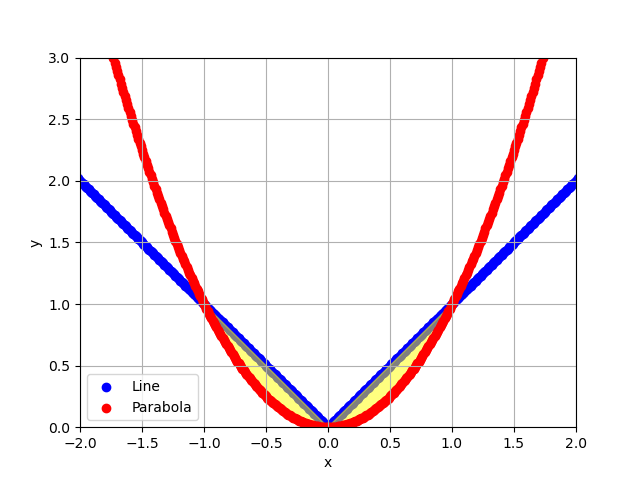
\includegraphics[width=1\columnwidth]{figs/fig.png}
   \caption{Graph of the parabola $y=x^2$ and $y=\abs{x}$ and the area enclosed between them}
   \label{stemplot}
\end{figure}
\end{document}
